\documentclass[a4paper,twocolumn]{article}
\usepackage[utf8]{inputenc}
\usepackage[margin=0.75in]{geometry}
\usepackage{graphicx}
\usepackage{amsmath}
\usepackage{enumerate} % Import the enumerate package
\usepackage{amsfonts}
\usepackage{hyperref}
\usepackage{float}
\usepackage{listings}
\usepackage{xcolor}
\usepackage{verbatim}


% Listings settings for Python code
\lstset{
    language=Python,
    basicstyle=\ttfamily\small,
    keywordstyle=\color{blue}\bfseries,
    stringstyle=\color{red},
    commentstyle=\color{green!70!black},
    numberstyle=\tiny\color{gray},
    numbers=left,
    stepnumber=1,
    numbersep=8pt,
    showspaces=false,
    showstringspaces=false,
    frame=single,
    breaklines=true,
    breakatwhitespace=true,
    tabsize=4,
    captionpos=b
}

\title{Emergency Response: Cooperation and Coordination Mechanisms in Multi-Agent Systems}
\author{Sheena Maria Lang, Antonio Lobo Santos, Zachary Parent, \\ María del Carmen Ramírez Trujillo and Bruno Sánchez Gómez}
\date{\today}

\begin{document}

\maketitle
\tableofcontents
\newpage

\section{Introduction}
% In this report, we propose a robust framework to address the emergency response problem using cooperation and coordination
%  mechanisms in multi-agent systems (MAS). The system, dubbed CrewAI, orchestrates diverse specialized crews to handle emergencies
%   through structured processes, ensuring efficiency, precision, and adaptability. The approach integrates process definition, 
%   pydantic outputs, and agent interaction, enabling smooth task execution and seamless inter-crew communication.
% \\

% The \textbf{process definition} outlines the workflows for individual crews, specifying sequential and parallel dependencies, agent roles,
%  and key operational details. Each crew is equipped with tailored processes to ensure timely and effective responses.
% \\ 

% \textbf{Pydantic outputs} ensure consistency and clarity by defining structured data models for task outputs. These models are
%  pivotal in facilitating inter-crew interactions and ensuring data integrity throughout the emergency response lifecycle.
% \\ 

% Finally, the \textbf{agent interaction} mechanism employs flow-based coordination, leveraging CrewAI’s advanced routing and state 
% management capabilities. Through logical operators and conditional triggers, the framework ensures synchronization across crews, 
% optimizing both task allocation and response accuracy.
% \\ 

% This comprehensive report details each component of the framework, emphasizing its adaptability and potential scalability, and leveraging insights from the literature \cite{app10155335, 2009-weiss, 10.5555/1695886}. 
% It serves as a blueprint for integrating multi-agent coordination into real-world emergency management systems.
% \\

% In the previous design process, we outlined the role of a \textbf{Forensics Team}, tasked with investigating the origins and causes 
% of fires. This team included a \textit{Forensics Operator}, who facilitated communication and updates with other emergency crews, 
% and a \textit{Forensics Coordinator}, responsible for managing team resources, assigning cases, and maintaining a database of current 
% and historical incidents. The \textit{Coroner} performed examinations of bodies at fire scenes and conducted detailed analyses in the 
% morgue, while the \textit{Investigator} handled on-site evidence collection, witness interviews, and cause determination. However, the 
% primary objective of this work was to develop a framework for emergency response planning rather than diving deeply into specific 
% scenarios or active interventions. As the forensic team’s functions extend beyond the immediate scope of emergency planning, it 
% has been excluded in order to maintain the focus on the core objectives.


\section{Process Definition}

\subsection{Emergency Services Crew}
\begin{enumerate}

    \item \textbf{Receive and Assess Call.} 
    The \textit{Emergency Call Agent} receives incoming calls and collects relevant details about the incident. 
    This task requires human input for accurate interpretation and contextual understanding of the caller's description, 
    ensuring critical information is gathered effectively. The information that this agent receives answers the following 
    six questions and is saved in a report:
    \begin{itemize}
        \item What type of fire is it? E.g. ordinary, electrical, gas, etc.
        \item Where is it? The location is received as coordinates \((x, y)\).
        \item Is anyone injured? How badly? The answer will be a list of strings, detailing the risk level of each person. If the list 
        if empty then there will be no injured people and it will be unnecessary to report it to the \textit{Medical Service Crew.}
        \item How severe is the fire? It will be considered as low, medium or high.
        \item Are there hazards? Examples of hazards could include gas cylinders, chemicals, explosions, etc.
        \item Is it an indoor or outdoor fire? The answer will be either \textit{outdoor} or \textit{indoor}.
        \item Is anyone inside or trapped? The answer will be an integer number $M$ representing the number of trapped people. 
        If $M > 0$, rescues are needed, and the \textit{Notification Agent} will detail that to the Fire Fighters Crew.
    \end{itemize}
    

    \item \textbf{Notify Other Crews Decision.} 
    The \textit{Notification Agent} receives the details about the fire then it decides which crew should be notify and send
    all the information to the flow. It also decides whether the medical services are required or not, depending on the 
    human input related to the injured individuals.    

\end{enumerate}

\paragraph{Task Dependencies:}

The sequential workflow for the Emergency Services Crew depends on task dependencies to ensure efficiency and coordination:
\begin{itemize}
    \item The \textit{Notify Other Crews Task} depends on the completion of the \textit{Receive and Assess Call Task}, which 
    involves human input to accurately assess and interpret the situation.
\end{itemize}


The task dependencies and agents who perform each task can be observed in Figure~\ref{fig:emergency_services_flow}.

\begin{figure}[h!]
	\centering
	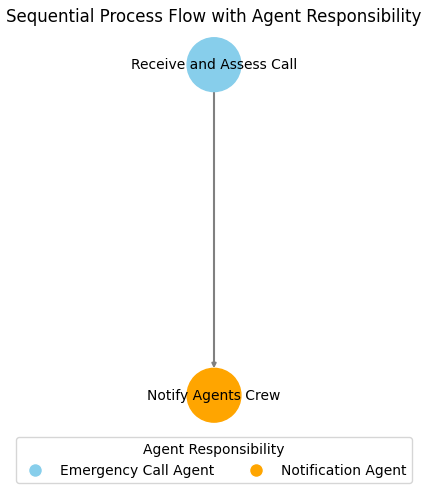
\includegraphics[height=0.4\textheight]{figures/emergency_services_crew_flow.png}
	\caption{Sequential Process Flow of the Medical Services Crew with Agent Responsibilities}
	\label{fig:emergency_services_flow}
\end{figure}

\subsection{Firefighter Agent Crew}

The Firefighter Agent Crew operates within a structured \textbf{sequential process} to ensure effective and coordinated response to fire emergencies. Each task is assigned to a specific agent with well-defined responsibilities, as detailed below:

\begin{enumerate}
    \item \textbf{Receive Report:} The \textit{Fire Chief} receives a fire assessment from the Emergency Service Operator. This serves as the starting point of the process, containing critical information such as the location and severity of the fire.
    \item \textbf{Allocate Firefighting Resources:} The \textit{Equipment Technician} determines if there exact resources required to combat the fire in question.
	\item \textbf{Deploy Fire Combatants:} The \textit{Fire Combatants} are deployed to the place of the fire, reporting an estimation of the time of arrival and a list of the fire fighting activities that will have to be performed.
	\item \textbf{Report Firefighting Response:} The \textit{Fire Chief} reports back a comprehensive summary of the firefighting activities.
\end{enumerate}

\paragraph{Task Dependencies}
The sequential process relies on strict task dependencies to maintain an organized workflow:
\begin{itemize}
    \item \textit{Allocate Firefighting Resources} depends on the completion of \textit{Receive Report}.
    \item \textit{Deploy Fire Combatants} depends on the completion of \textit{Deploy Fire Combatants}.
    \item \textit{Report Firefighting Response} depends on the completion of \textit{Deploy Fire Combatants}.
\end{itemize}

The visual representation in Figure~\ref{fig:firefighter_flow} highlights these dependencies and assigns colors to denote the responsible agents.

\begin{figure}[ht!]
	\centering
	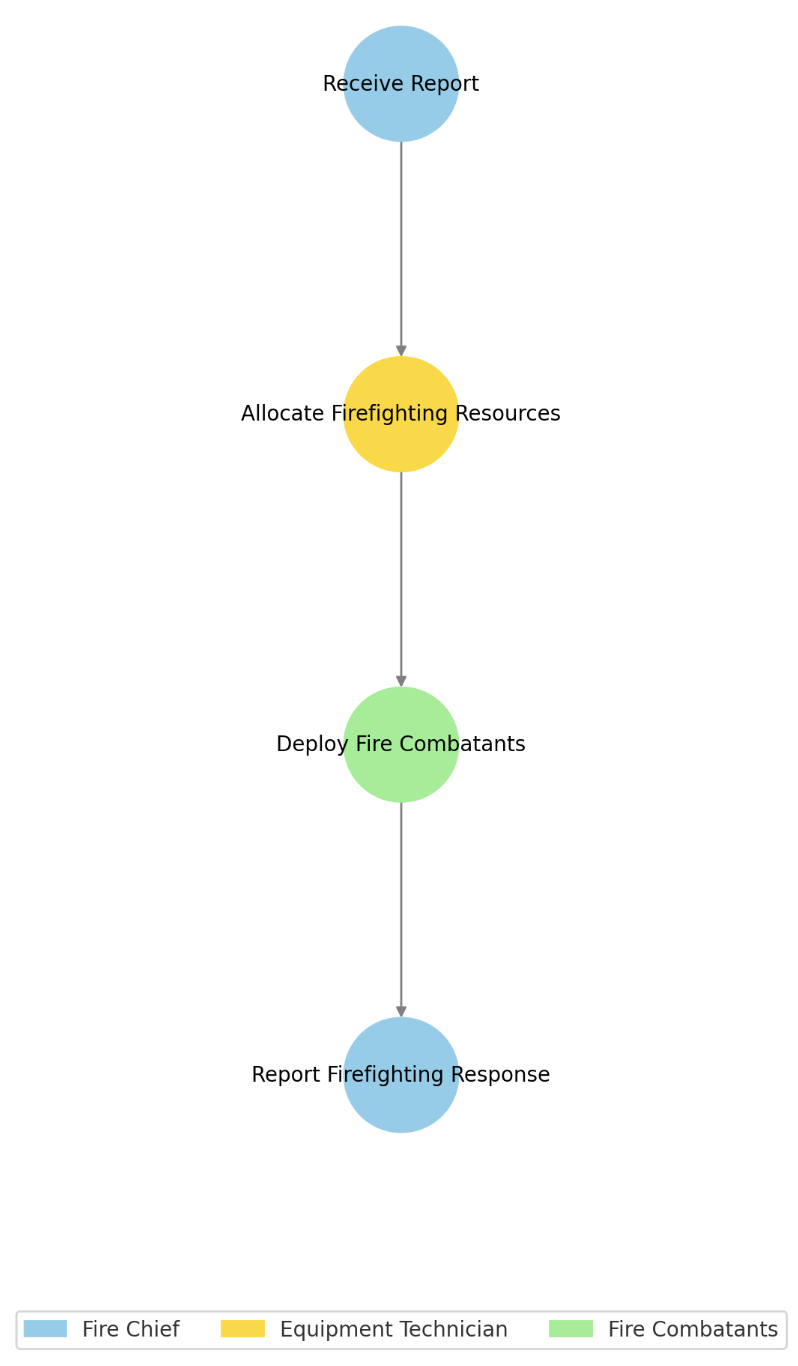
\includegraphics[height=0.59\textheight]{figures/Firefighter_Crew_Flow.png}
	\caption{Sequential Process Flow of the Firefighter Crew with Agent Responsibilities}
	\label{fig:firefighter_flow}
\end{figure}

\subsection{Medical Services Crew}

The Medical Services Crew operates follows a \textbf{sequential} task structure to plan the treatment and evacuation of injured people from the emergency site. The tasks included within the Medical Services are:

\begin{enumerate}
	\item \textbf{Receive Report:} The \textit{Medical Services Operator} receives the medical assessment of the fire incident, and parses key information, such as the location, the number of injured, and the severity of injuries.
	
	\item \textbf{Rank Hospitals:} The \textit{Hospital Coordinator} ranks the city's hospitals based on distance to the emergency location.

	\item \textbf{Allocate Hospital Resources:} The \textit{Hospital Coordinator} assesses the available resources (beds, ambulances, paramedics) at the hospitals, and allocates their resources according to the needs of the emergency.
	
	\item \textbf{Deploy Paramedics:} The \textit{Paramedics} plan their deployment to the place of the incident, reporting the total number of paramedics and ambulances dispatched, as well as their estimated times of arrival, and any special equipment that they could need.
	
	\item \textbf{Report Medical Response:} The \textit{Medical Services Operator} reports back a comprehensive summary of the response plan.
\end{enumerate}

\paragraph{Task Dependencies}
The sequential nature of the process requires to establish task dependencies to define the crew's workflow:
\begin{itemize}
	\item The \textit{Rank Hospitals} task depends on the completion of the \textit{Recieve Report} task.
	\item The \textit{Allocate Hospital Resources} task depends on the completion of \textit{Rank Hospitals}.
	\item The \textit{Deploy Paramedics} task depends on the completion of \textit{Allocate Hospital Resources}.
	\item The \textit{Report Medical Response} task depends on the completion of \textit{Deploy Paramedics}.
\end{itemize}

The task dependencies and agents who perform each task can be observed in Figure~\ref{fig:medical_services_flow}.

\begin{figure}[ht!]
	\centering
	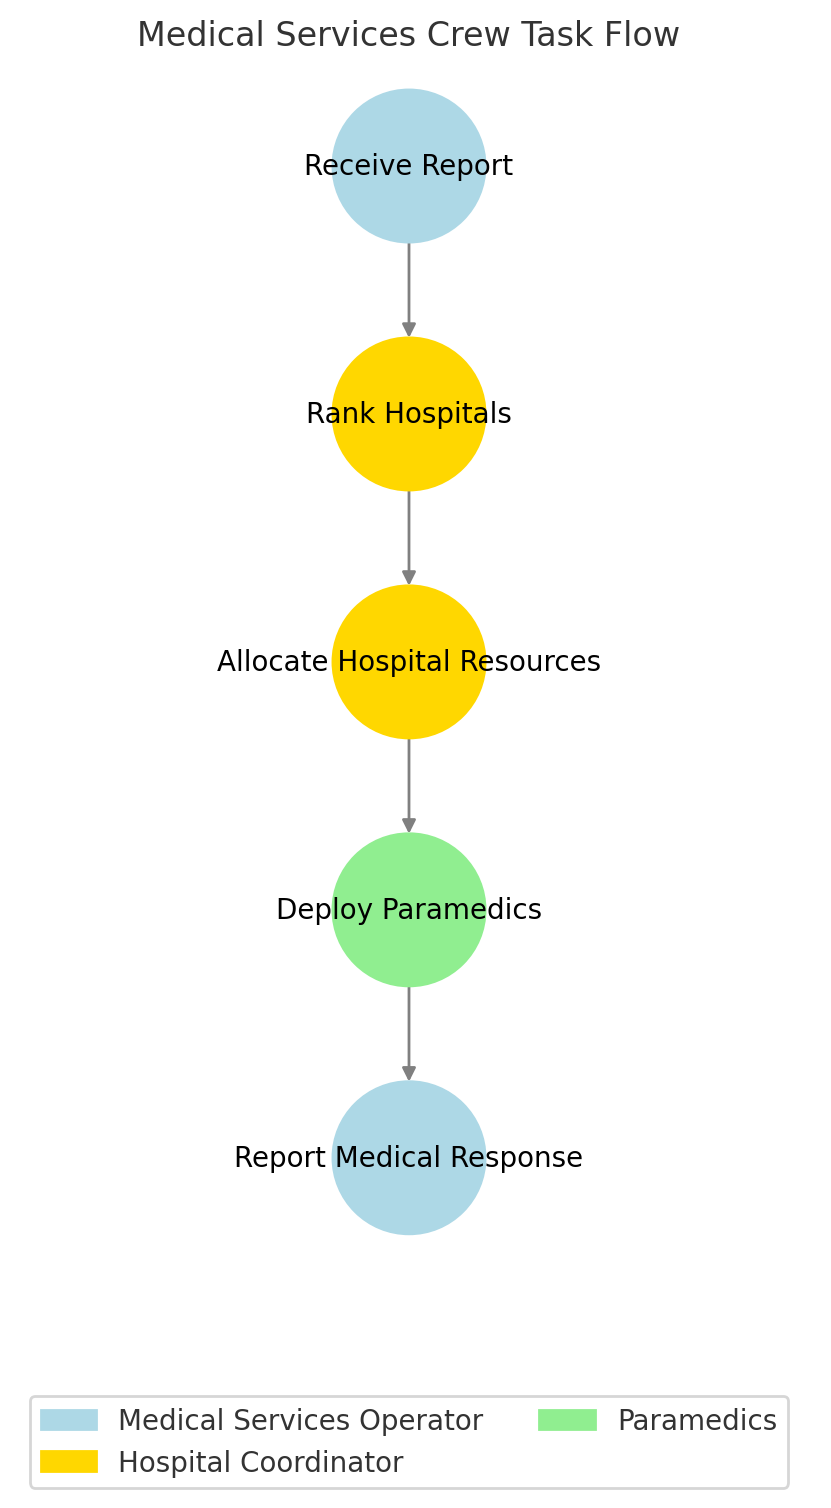
\includegraphics[height=0.6\textheight]{figures/Medical_Services_Crew_Flow.png}
	\caption{Sequential Process Flow of the Medical Services Crew with Agent Responsibilities}
	\label{fig:medical_services_flow}
\end{figure}

\subsection{Public Communication Crew}

The Public Communication Crew operates within a structured \textbf{sequential process} to ensure efficient and accurate communication of fire incident reports to the public. Each task is assigned to a specific agent with well-defined responsibilities, as detailed below:

\begin{enumerate}
	\item \textbf{Receive Report:} The \textit{Communication Operator} obtains the call assessment, fire report, and medical report in Markdown format. This serves as the starting point for the process and can filter any information that is not relevant for this crew.
	\item \textbf{Search Related Cases:} The \textit{Archive Keeper} searches for past incidents with similar locations or fire types. This task depends on the completion of the \textit{Receive Report} task.
	\item \textbf{Draft Initial Article:} The \textit{Article Writer} drafts an initial article based on the current report. This task also depends on the completion of the \textit{Receive Report} task.
	\item \textbf{Integrate Additional Information:} The \textit{Article Writer} integrates insights from related cases into the draft. This task requires the completion of both the \textit{Search Related Cases} and \textit{Draft Initial Article} tasks.
	\item \textbf{Review and Authorize Publication:} The \textit{Mayor} reviews the article and either authorizes publication or provides feedback for revisions. This task depends on the completion of the \textit{Integrate Additional Information} task.
	\item \textbf{Provide Social Media Feedback:} The \textit{Social Media Commentator} critiques the emergency response in a humorous yet constructive manner. This task depends on the approval of the article by the \textit{Mayor}.
\end{enumerate}

\begin{figure}[ht!]
	\centering
	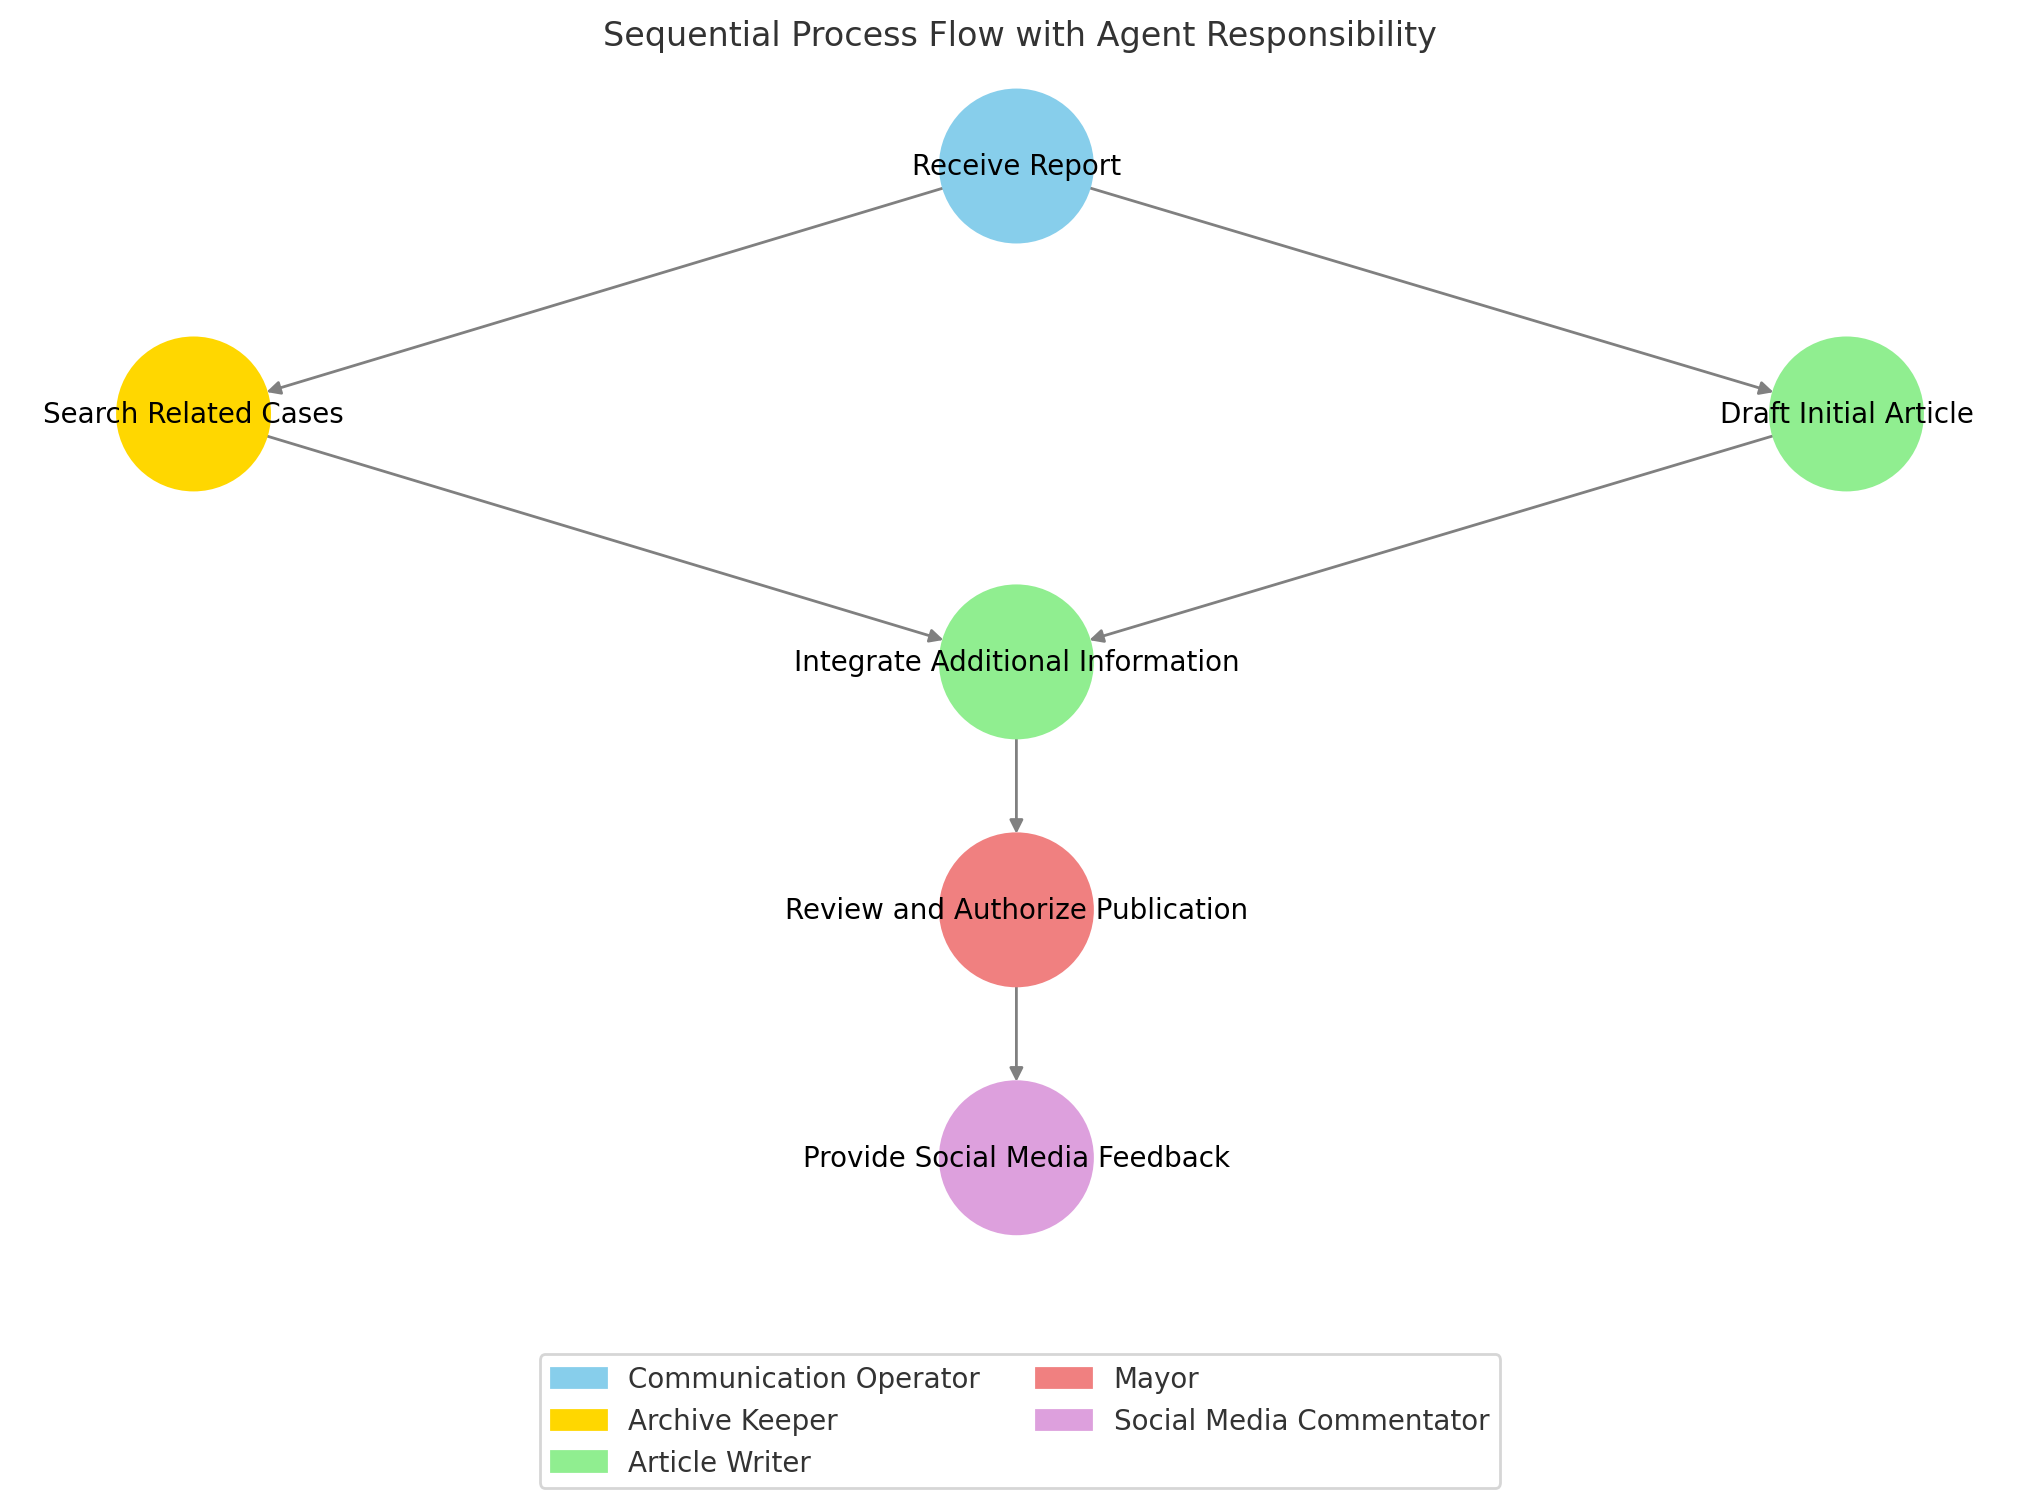
\includegraphics[width=0.4\textwidth]{figures/PC-process.png}
	\caption{Sequential Process Flow of the Public Communication Crew with Agent Responsibilities}
	\label{fig:public_comm_flow}
\end{figure}


\paragraph{Task Dependencies}
The sequential process relies on strict task dependencies to ensure an organized workflow:
\begin{itemize}
	\item \textit{Search Related Cases} and \textit{Draft Initial Article} can be executed in parallel but both depend on \textit{Receive Report}.
	\item \textit{Integrate Additional Information} requires the completion of both \textit{Search Related Cases} and \textit{Draft Initial Article}.
	\item \textit{Review and Authorize Publication} depends on \textit{Integrate Additional Information}.
	\item \textit{Provide Social Media Feedback} requires article approval from the \textit{Mayor}.
\end{itemize}

The visual representation in Figure~\ref{fig:public_comm_flow} highlights these dependencies and assigns colors to denote the responsible agents, ensuring clarity and accountability.




\section{Pydantic Outputs}
Structured outputs are essential for ensuring clarity and consistency in task execution. Below are listed the Pydantic models used in the system.

\subsection{Pydantic Outputs for Public Communication Crew}

Structured outputs are crucial for ensuring clarity, consistency, and seamless integration across tasks. Below are the Pydantic models designed for the tasks in the Public Communication Crew process:

\subsubsection{Receive Report Task Output}
\begin{lstlisting}[caption={Pydantic model for Receive Report Task Output}]
from pydantic import BaseModel

class ReceiveReportOutput(BaseModel):
    report_id: str
    location: str
    fire_type: str
    timestamp: str
    markdown_content: str
\end{lstlisting}

\subsubsection{Search Related Cases Task Output}
\begin{lstlisting}[caption={Pydantic model for Search Related Cases Task Output}]
from pydantic import BaseModel
from typing import List

class RelatedCase(BaseModel):
    case_id: str
    location: str
    fire_type: str
    summary: str

class SearchRelatedCasesOutput(BaseModel):
    related_cases: List[RelatedCase]
    total_cases: int
\end{lstlisting}

\subsubsection{Draft Initial Article Task Output}
\begin{lstlisting}[caption={Pydantic model for Draft Initial Article Task Output}]
from pydantic import BaseModel

class DraftArticleOutput(BaseModel):
    title: str
    draft: str
    author: str
\end{lstlisting}

\subsubsection{Integrate Additional Information Task Output}
\begin{lstlisting}[caption={Pydantic model for Integrate Additional Information Task Output}]
from pydantic import BaseModel

class IntegratedArticleOutput(BaseModel):
    draft: str
    integrated_sources: list[str]
\end{lstlisting}

\subsubsection{Review and Authorize Publication Task Output}
\begin{lstlisting}[caption={Pydantic model for Review and Authorize Publication Task Output}]
from pydantic import BaseModel

class ReviewOutput(BaseModel):
    approved: bool
    comments: str
    draft: str
\end{lstlisting}

\subsubsection{Provide Social Media Feedback Task Output}
\begin{lstlisting}[caption={Pydantic model for Provide Social Media Feedback Task Output}]
from pydantic import BaseModel

class SocialMediaFeedbackOutput(BaseModel):
    feedback: str
    draft: str
    approved: bool
    comments: str
\end{lstlisting}

\paragraph{Summary of Outputs}
\begin{itemize}
    \item \textbf{Receive Report Task Output:} Captures the initial fire incident report relevant details.
    \item \textbf{Search Related Cases Task Output:} Retrieves relevant historical cases for contextualization.
    \item \textbf{Draft Initial Article Task Output:} Records the initial draft content.
    \item \textbf{Integrate Additional Information Task Output:} Updates the draft with integrated sources and revisions.
    \item \textbf{Review and Authorize Publication Task Output:} Specifies the review status and comments from the Mayor.
    \item \textbf{Provide Social Media Feedback Task Output:} Details feedback posted on social media platforms, he can critize the mayor's decission.
\end{itemize}



\section{Crew Interactions and Flow}
\label{sec:crew_interaction}

\subsection{Flow Design and Coordination}
The Emergency Planner Flow is designed to handle emergency situations by coordinating multiple crews. The flow begins with the retrieval of a call transcript, followed by the processing of the call by emergency services. Based on the assessment, firefighters and medical services are dispatched in parallel. Public communication is managed after both teams report or during approval retries. Once the emergency is resolved, the flow concludes with the generation of a comprehensive emergency report, which includes summaries and timestamps from all participating crews.

\subsubsection{State Management}
The system maintains a centralized state using a Pydantic model \footnote{\url{https://docs.crewai.com/concepts/flows\#structured-state-management}}, `EmergencyPlannerState`, which tracks all aspects of the emergency response. This includes the call transcript, assessments, and response reports. The state model ensures type-safe storage and accommodates partial updates.

\subsection{Technical Implementation}
The flow is orchestrated using CrewAI's decorators, which define the sequence and conditions for crew operations. Key flow control points include:

\begin{itemize}
    \item \texttt{@start()}\footnote{\url{https://docs.crewai.com/concepts/flows\#start}} for initiating the call transcript retrieval.
    \item \texttt{@listen()}\footnote{\url{https://docs.crewai.com/concepts/flows\#listen}} for establishing dependencies between operations, such as emergency services processing and the dispatch of firefighters and medical services.
    \item \texttt{@router()}\footnote{\url{https://docs.crewai.com/concepts/flows\#router}} for handling conditional flow control, particularly for public communication approval.
\end{itemize}


\subsubsection{Router Implementation}
The router manages public communication approval, checking if the mayor has approved the communication. If not, it retries up to a maximum count. This ensures that public communication is handled appropriately and efficiently.
This includes the use of \texttt{and\_} and \texttt{or\_} to combine multiple conditions. This is key for the retry mechanism for public communication approval.

\paragraph{Complex Logic for Public Communications}
\texttt{and\_} \footnote{\url{https://docs.crewai.com/concepts/flows\#conditional-logic-and}} and \texttt{or\_} \footnote{\url{https://docs.crewai.com/concepts/flows\#conditional-logic-or}} are used to combine multiple conditions. This is key for the retry mechanism for public communication approval.

\begin{lstlisting}[language=Python]
@listen(or_(and_(firefighters, medical_services), "retry_public_communication"))
def public_communication(self):
    # ...
\end{lstlisting}

\paragraph{Router Logic for Public Communication Approval}
The router emits different messages based on the conditions, either triggering a retry or saving the full emergency report.

\begin{lstlisting}[language=Python]
@router(public_communication)
def check_approval(self):
    logger.info("Checking approval")
    if self.state.public_communication_report.mayor_approved:
        return "save full emergency report"
    elif self.state.mayor_approval_retry_count >= MAX_MAYOR_APPROVAL_RETRY_COUNT:
        return "save full emergency report"
    self.state.mayor_approval_retry_count += 1
    return "retry_public_communication"
\end{lstlisting}

\subsection{Justification of Design Choices}
The design choices are justified by the need for a robust and flexible system that can handle complex emergency scenarios. The use of CrewAI's flow decorators allows for clear and maintainable code, while the parallel processing capabilities ensure timely responses from different crews.



\section{Conclusion}
% This report presents a comprehensive multi-agent system for emergency response coordination, implementing sophisticated cooperation mechanisms across specialized crews. The key achievements and insights include:

% \begin{itemize}
%     \item \textbf{Process Definition:} Each crew operates with clearly defined sequential workflows:
%     \begin{itemize}
%         \item Emergency Services established structured protocols for initial assessment and crew dispatch
%         \item Firefighters implemented systematic resource allocation and deployment procedures
%         \item Medical Services developed efficient hospital ranking and resource coordination
%         \item Public Communications created an iterative approval workflow with historical case integration
%     \end{itemize}
    
%     \item \textbf{Data Standardization:} Implementation of Pydantic models ensures:
%     \begin{itemize}
%         \item Type-safe data transfer between crews
%         \item Consistent reporting formats
%         \item Structured storage of emergency response states
%     \end{itemize}
    
%     \item \textbf{Coordination Mechanisms:} The system achieves efficient crew interaction through:
%     \begin{itemize}
%         \item Centralized state management
%         \item Parallel processing capabilities
%         \item Sophisticated routing mechanisms
%         \item Retry systems for critical operations
%     \end{itemize}
% \end{itemize}

% The framework demonstrates the effectiveness of structured agent cooperation in emergency response scenarios. Future work could explore the integration of additional specialized crews (such as Forensics) and further optimization of the coordination mechanisms for larger-scale emergencies.

\section{References}
\bibliography{references}
\bibliographystyle{plain}
\end{document}
